\documentclass[10pt,twocolumn]{article}
\usepackage[a4paper,margin=0.72in]{geometry}
\usepackage[T1]{fontenc}
\usepackage{lmodern}
\usepackage{microtype}
\usepackage{amsmath,amssymb}
\usepackage{booktabs}
\usepackage{tabularx}
\usepackage{graphicx}
\usepackage{caption}
\usepackage{subcaption}
\usepackage[numbers,sort&compress]{natbib}
\usepackage{xurl}
\usepackage{hyperref}
\hypersetup{colorlinks=true,linkcolor=black,citecolor=blue,urlcolor=blue}
\graphicspath{{figures/}}
\newcommand{\cmaps}{C-MAPSS}
\newcommand{\rul}{RUL}
\newcommand{\duallstm}{Dual-LSTM}
\title{\textbf{Cycle-Consistent Safety-Oriented Dual-LSTM for Aero-Engine Remaining Useful Life Prediction}}
\author{Ethan Huang\\Beihang University}
\date{June 28, 2026}
\begin{document}
\maketitle

\begin{abstract}
Remaining useful life (RUL) models for aero-engines are often selected by aggregate accuracy, although late-life overestimation has a different maintenance meaning from conservative underestimation. This paper tests a cycle-consistent safety-oriented Dual-LSTM as a method response to the RMSE/risk-ranking discordance observed under a safety-oriented C-MAPSS protocol. The model augments a current-window LSTM RUL branch with a target-conditioned degradation-transition branch during training; future same-engine windows are used only as regularization signals, while inference uses only the current last window. Across FD001--FD004 with three seeds, cycle consistency changed RMSE relative to the LSTM baseline by -4.6\% to +0.4\%. Adding safety weighting to the cycle branch reduced Critical RMSE50 by -21.3\% to -7.5\% and overestimation magnitude by -42.6\% to -29.1\% relative to cycle-only Dual-LSTM. Paired seed-engine bootstrap checks show that the overestimation-magnitude reduction is supported on all four subsets, whereas RMSE gains from cycle consistency are weaker. The contribution is therefore a bounded risk-profile shaping method under a simulated benchmark protocol, not a universal state-of-the-art architecture or aviation safety certification result.
\end{abstract}

\noindent\textbf{Keywords:} remaining useful life; C-MAPSS; turbofan engine; Dual-LSTM; cycle consistency; safety-oriented evaluation; overestimation risk

\section{Introduction}
Remaining useful life (RUL) prediction estimates how many operating cycles remain before a component reaches failure. In prognostics and health management, RUL estimates support inspection planning, spare-parts allocation, and maintenance scheduling for high-value assets \citep{Jardine2006}. For aero-engine settings, however, prediction errors are not operationally symmetric. Conservative underestimation can waste useful life, whereas optimistic overestimation may delay maintenance action and is therefore the more safety-relevant failure mode.

NASA C-MAPSS is a standard simulation benchmark for aero-engine degradation and RUL prediction \citep{NASA_PCoE,Saxena2008}. Early deep studies established convolutional and recurrent sequence models for C-MAPSS RUL prediction \citep{Babu2016,Zheng2017,Li2018}, and later work introduced temporal convolution, attention, Transformer, Koopman, Bayesian, and decision-aware variants \citep{Liu2023SAETCN,Fan2024STAR,Kim2025KoopmanTransformer,Hu2023Bayesian,Xiang2024BayesianGated,DePater2022,Mitici2023}. These studies improve representation or downstream use, but they often leave a narrower model-selection question unresolved: whether the model favored by aggregate RMSE is also favored by late-life error and optimistic-risk metrics.

This paper builds directly on that evaluation gap. Rather than proposing another large architecture family, we ask whether a lightweight dual recurrent structure can reshape the error distribution under the same safety-oriented protocol. Long short-term memory networks provide the recurrent backbone \citep{Hochreiter1997,Zheng2017}. The dual-branch idea is inspired by consistency-driven dual recurrent modeling in another sequential-control domain \citep{DualLSTMSoftRobot2026}, but C-MAPSS lacks control inputs, so we do not transfer an inverse-control interpretation. Instead, we use a current-window RUL branch and a target-conditioned degradation-transition branch trained with cycle and latent consistency, conceptually related to cycle-consistency regularization \citep{Zhu2017CycleGAN}.

The contributions are threefold. First, we formalize a cycle-consistent Dual-LSTM for C-MAPSS RUL prediction in which future windows are training-only regularization signals. Second, we evaluate LSTM, Dual-LSTM no-cycle, Dual-LSTM cycle, and Dual-LSTM cycle+safety-w2 across FD001--FD004 with three seeds. Third, we connect Paper 2 back to the Paper 1 safety benchmark by reporting RMSE, MAE, NASA score, Critical RMSE30/50, overestimation ratio, overestimation magnitude, paired seed-engine bootstrap, and a bridge against the representative Paper 1 portfolio.

\section{Methods}
\subsection{Data and protocol}
We use FD001--FD004 of the NASA C-MAPSS benchmark \citep{NASA_PCoE,Saxena2008}. Training trajectories run to failure, and test trajectories are truncated with official final RUL labels. We use engine-level validation splits, train-only scaling, a maximum RUL cap of 130 cycles, 30-cycle windows, and last-window test evaluation. The seeds are 42, 43, and 44. These choices match the Paper 1 safety-oriented evaluation protocol so that Paper 2 functions as a method-response experiment rather than a protocol-tuning study.

\subsection{Paired-window Dual-LSTM}
For each engine, same-engine paired windows are constructed as $(X_t,y_t,X_{t+k},y_{t+k},k)$ with $k=1$. The current branch maps $X_t$ to a latent state $z_t$ and predicts $\hat{y}_t$. The transition branch receives $z_t$ and horizon $k$ and predicts a future latent state $\hat{z}_{t+k}$, which is passed through the RUL head to predict $\hat{y}_{t+k}$. Latent consistency aligns $\hat{z}_{t+k}$ with a stop-gradient encoding of $X_{t+k}$, and a monotonic penalty discourages future predicted RUL from exceeding current predicted RUL. At inference time, only the current-window branch is used.

\subsection{Losses and evaluation}
The cycle-only job uses current RUL loss, future-cycle loss, latent consistency, and monotonic regularization. The safety-w2 job additionally uses the existing safety-weighted loss to emphasize critical-zone and optimistic-overestimation errors. We report RMSE, MAE, NASA score, Critical RMSE30/50, overestimation ratio, and overestimation magnitude. For robustness, we use paired bootstrap over seed-engine rows, pairing two jobs on the same subset, seed, and test engine. Lower metric values are better throughout.

\section{Results}
\subsection{Full matrix integrity}
The full Paper 2 matrix contains 48 complete jobs: four subsets, three seeds, and four jobs. Each job has metrics, predictions, training history, and selected-feature outputs. The aggregated metric table contains 96 rows over validation and test splits, and every subset/job/split has exactly three seeds.

\subsection{Cycle consistency gives a modest representation signal}
Cycle-only Dual-LSTM improved RMSE relative to the LSTM baseline on three of four subsets by point estimate, with changes ranging from -4.6\% to +0.4\%. However, paired bootstrap intervals exclude zero for only one of four subset-level RMSE contrasts, so this result should be described as a modest representation signal rather than a decisive RMSE win (Table~\ref{tab:cycle}).

\begin{table*}[t]
\centering
\caption{Cycle-only Dual-LSTM versus LSTM baseline. Values are candidate minus baseline. Negative values indicate lower error for cycle-only Dual-LSTM.}
\label{tab:cycle}
\small
\begin{tabular}{lrrrr}
\toprule
Subset & RMSE change & RMSE diff & 95\% CI & Bootstrap \\
\midrule
FD001 & -0.8\% & -0.13 & [-0.91, 0.65] & uncertain \\
FD002 & -1.8\% & -0.33 & [-1.05, 0.33] & uncertain \\
FD003 & +0.4\% & 0.06 & [-1.09, 1.17] & uncertain \\
FD004 & -4.6\% & -1.08 & [-1.97, -0.31] & improvement \\
\bottomrule
\end{tabular}
\end{table*}

\subsection{Safety weighting shifts optimistic-risk behavior}
The strongest Paper 2 result is not aggregate RMSE. Cycle+safety-w2 reduced Critical RMSE50 on all four subsets by point estimate, with relative changes from -21.3\% to -7.5\%. It also reduced overestimation magnitude on all four subsets, with changes from -42.6\% to -29.1\%; the overestimation-magnitude bootstrap interval excludes zero on all four subsets (Table~\ref{tab:safety}). FD002 is the main trade-off case: risk metrics improve, but RMSE increases relative to cycle-only Dual-LSTM.

\begin{table*}[t]
\centering
\caption{Cycle+safety-w2 versus cycle-only Dual-LSTM. Relative changes are computed from three-seed test means. The final column gives the paired-bootstrap 95\% CI for overestimation-magnitude difference.}
\label{tab:safety}
\small
\begin{tabular}{lrrrr}
\toprule
Subset & RMSE & Critical RMSE50 & OverMag & OverMag 95\% CI \\
\midrule
FD001 & +0.2\% & -9.5\% & -42.6\% & [-3.78, -2.51] \\
FD002 & +12.5\% & -7.5\% & -30.3\% & [-2.04, -1.33] \\
FD003 & -2.7\% & -20.9\% & -29.1\% & [-2.57, -1.28] \\
FD004 & +0.3\% & -21.3\% & -33.7\% & [-3.63, -2.49] \\
\bottomrule
\end{tabular}
\end{table*}

\begin{figure*}[t]
\centering
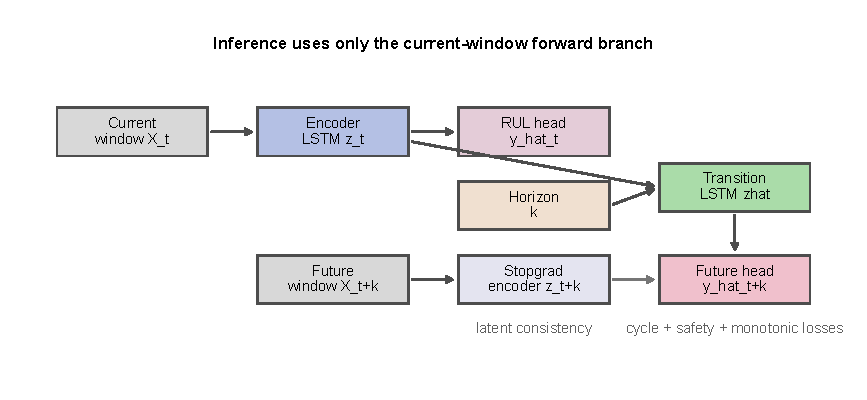
\includegraphics[width=0.95\textwidth]{figure_01_dual_lstm_architecture.pdf}
\caption{Cycle-consistent Dual-LSTM architecture. The current-window branch predicts test-time RUL. The future-window branch is used only during training through cycle, latent-consistency, monotonic, and optional safety-weighted losses.}
\label{fig:architecture}
\end{figure*}

\begin{figure*}[t]
\centering
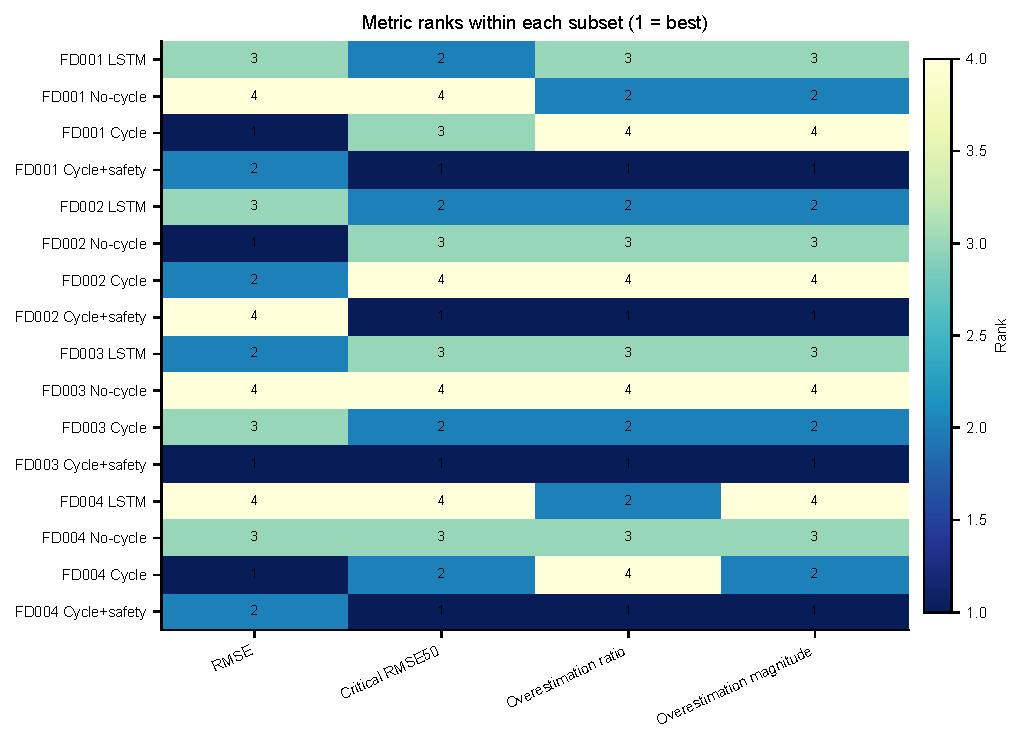
\includegraphics[width=0.88\textwidth]{figure_02_dual_lstm_metric_rank_heatmap.pdf}
\caption{Metric ranks across FD001--FD004. Rank 1 is best within a subset and metric. The heatmap shows that aggregate RMSE and risk-oriented metrics do not always select the same job.}
\label{fig:rank}
\end{figure*}

\begin{figure*}[t]
\centering
\begin{subfigure}[t]{0.49\textwidth}
\centering
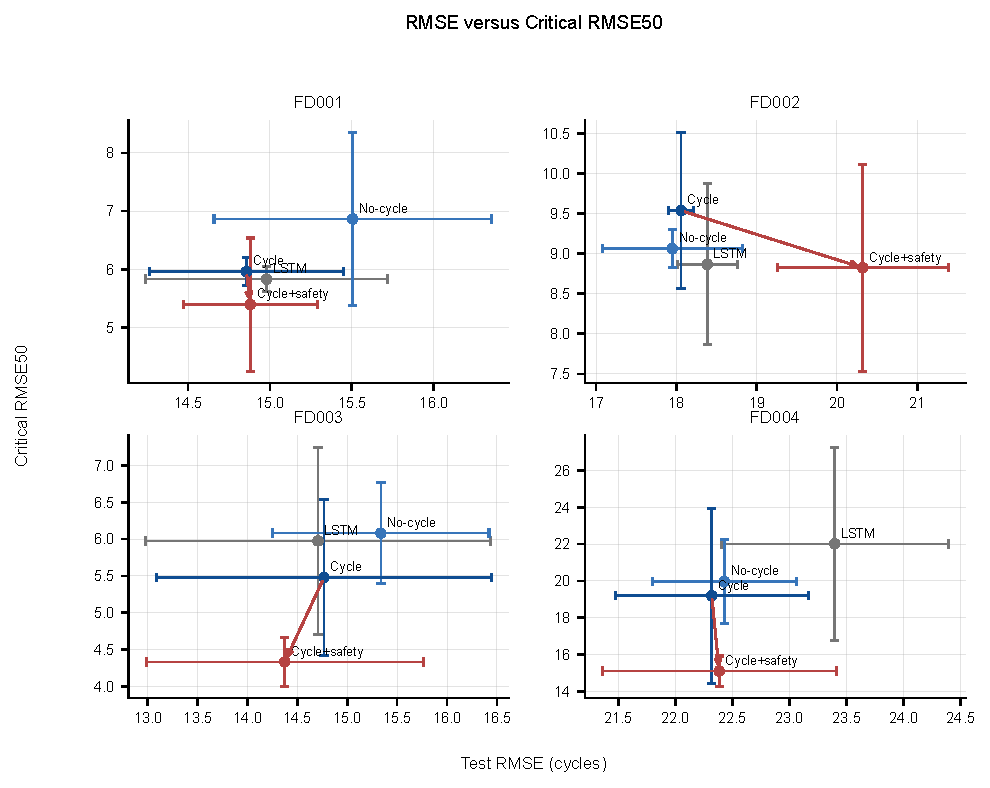
\includegraphics[width=\linewidth]{figure_03_rmse_vs_critical_rmse50.pdf}
\caption{Critical RMSE50 trade-off.}
\end{subfigure}
\begin{subfigure}[t]{0.49\textwidth}
\centering
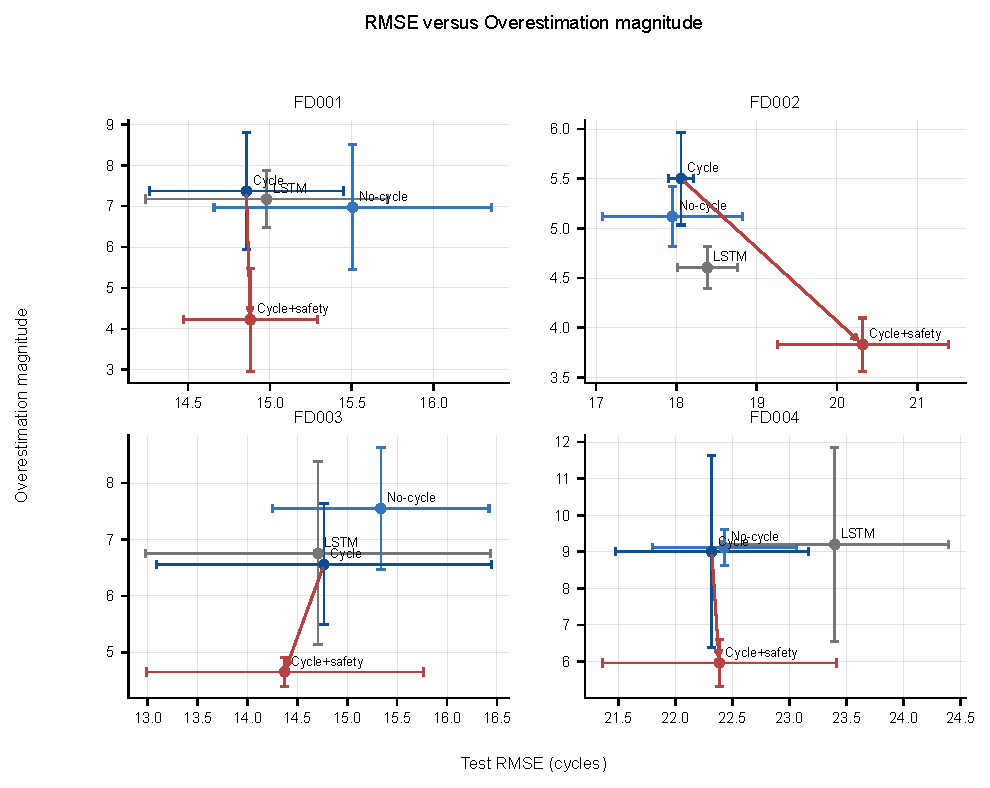
\includegraphics[width=\linewidth]{figure_04_rmse_vs_overestimation_magnitude.pdf}
\caption{Overestimation-magnitude trade-off.}
\end{subfigure}
\caption{RMSE-risk trade-off plots. Arrows show the movement from cycle-only Dual-LSTM to cycle+safety-w2. Safety weighting generally moves the model toward lower risk metrics, with subset-dependent RMSE cost.}
\label{fig:tradeoff}
\end{figure*}

\subsection{Paper 1 bridge limits the claim}
Compared with the Paper 1 representative-matrix best result, the best Paper 2 job is lower in 4/20 subset-metric cells. This bridge is useful because it prevents overclaiming: Dual-LSTM is a risk-profile shaping candidate under the Paper 1 protocol, not a replacement for strong classical baselines or the full GRU safety-ablation portfolio.

\begin{figure*}[t]
\centering
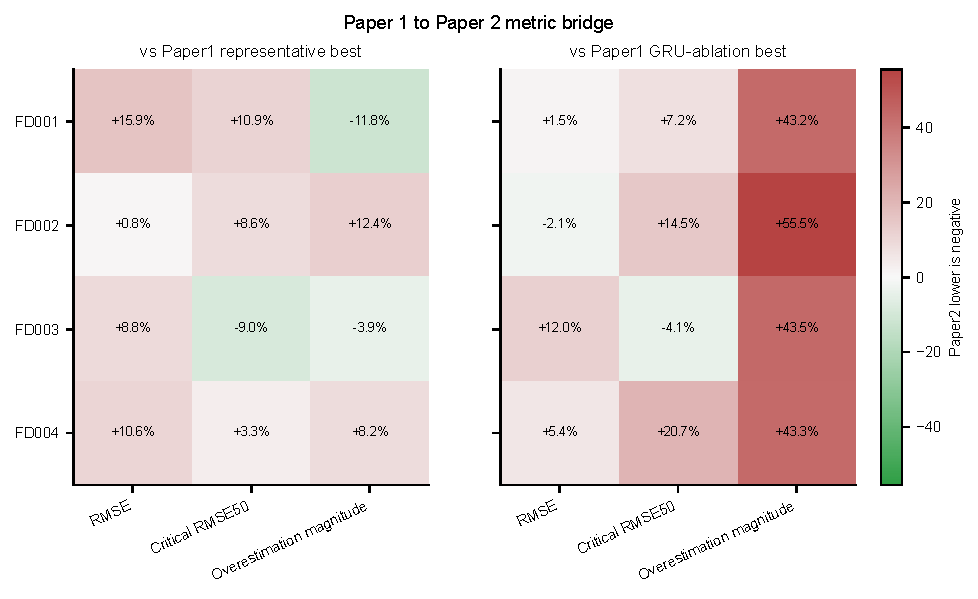
\includegraphics[width=0.92\textwidth]{figure_05_paper1_paper2_bridge.pdf}
\caption{Paper 1 to Paper 2 bridge. Negative values indicate that the best Paper 2 job is lower than the corresponding Paper 1 best value for that subset and metric. The sparse green cells support a bounded method-response interpretation rather than a full-portfolio SOTA claim.}
\label{fig:bridge}
\end{figure*}

\section{Discussion}
The experiments support a narrow but useful conclusion. Cycle consistency appears to provide a modest representation signal, but the RMSE evidence is not strong enough to make cycle-only Dual-LSTM a universal accuracy winner. Safety weighting, by contrast, consistently reduces optimistic-risk behavior, especially overestimation magnitude, across all four subsets. This is exactly the type of finding suggested by the Paper 1 safety benchmark: a model intervention may be valuable because it changes the error distribution, even when it does not dominate aggregate RMSE.

The main limitations are also clear. First, the LSTM baseline trains on all sequence windows, whereas Dual-LSTM jobs train on paired windows that require a future same-engine window. The comparison therefore reflects branch, loss, and protocol differences, not a pure parameter-count comparison. Second, the bootstrap resamples simulated seed-engine rows and should not be interpreted as real-fleet safety evidence. Third, three seeds are useful for stability screening but still modest. Finally, C-MAPSS does not include real maintenance costs, scheduling constraints, or aviation certification requirements, so the safety terminology here refers to benchmark risk metrics only.

\section{Conclusion}
Cycle-consistent safety-oriented Dual-LSTM is a viable Paper 2 candidate under the C-MAPSS safety-evaluation protocol. Its strongest evidence is systematic reduction of overestimation magnitude when safety weighting is added to the cycle branch, while RMSE effects remain subset-dependent. The paper should therefore be positioned as a method-response and risk-profile shaping study, not as a universal SOTA model paper.

\section*{Data and Code Availability}
The experiments use the public NASA C-MAPSS dataset. Paper-facing CSV outputs, figure source tables, and scripts are provided in the project repository. Generated model weights and full prediction tables are treated as reproducible experiment artifacts and can be regenerated from the documented commands.

\section*{Acknowledgements}
This manuscript draft was prepared as part of an internal C-MAPSS RUL research workflow. All claims should be checked against the accompanying CSV and source-code trace before external submission.

\bibliographystyle{unsrtnat}
\bibliography{references}
\end{document}
